\documentclass[11pt]{article}
\usepackage{graphicx}
\usepackage{hyperref}
\usepackage{appendix}
\usepackage{amsmath}
\usepackage{amssymb}
\usepackage{float}
\usepackage{commath}
\usepackage{siunitx}
\sisetup{detect-all}
\usepackage[a4paper,margin=20mm]{geometry}
\numberwithin{equation}{section}
\setlength{\parskip}{\baselineskip}%
\setlength{\parindent}{0pt}%
\hypersetup{
    colorlinks=true,
    linkcolor=magenta,
    filecolor=magenta,      
    urlcolor=magenta,
}
\urlstyle{same}
\begin{document}
\title{\textbf{UCL Mechanical Engineering 2020/2021}\\ENGF0004 Open Book Exam 1}
\author{NCWT3}
\maketitle
\section{Question 1}
\subsection*{a}
Boundary conditions
\begin{gather}
  \left.\frac{dx}{dt}\right|_{t=0} = v, \ x(0) = k
\end{gather}
Laplace transform:
\begin{gather}
  \frac{d^2 x}{d t^2} + 2p\omega_0\frac{d x}{d t} + \omega_0^2 = 0\\
  s^2 X(s) - sX(0) - X'(0) + 2p\omega_0 s X(s) - 2p\omega_0 X(0) + \omega_0^2 X(s) = 0\\
  X(s) \left(s^2 - 2p\omega_0 + \omega_0^2\right) -s X(0) - X'(0)-2p\omega_0X(0) = 0
\end{gather}
\begin{align}
  X(s) \left(s^2 - 2p\omega_0 + \omega_0^2\right) &= sk + v + 2p\omega_0 k\\
  X(s) &= \frac{sk + v + 2p\omega_0 k}{s^2 - 2p\omega_0 + \omega_0^2}
\end{align}
\subsection*{b}
Completing the square
\begin{gather}
  s^2 + 2 p \omega_0 + \omega_0^2\\
  (s + p\omega_0)^2 + \omega_0^2 - p^2\omega_0^2
\end{gather}
Substituting:
\begin{align}
  X(s) &= \frac{ks + v + sp\omega_0 k}{(s + p\omega_0 )^2 + \omega_0^2(1-p^2)}\\
  X(s) &= \frac{-\frac{sv}{p\omega_0} + v -\frac{2p\omega_0 v}{p \omega_0}}{(s + p\omega_0 )^2 + \omega_0^2(1-p^2)}\\
  X(s) &= \frac{-\frac{sv}{p\omega_0} -v}{(s + p\omega_0 )^2 + \omega_0^2(1-p^2)}\\
  X(s) &= -\frac{v}{p\omega_0} \cdot \frac{s+ p \omega_0}{(s + p\omega_0 )^2 + \omega_0^2(1-p^2)}\\
\end{align}
From Laplace table:
\begin{gather}
  x(t) = -\frac{v}{p\omega_0} e^{-p\omega_0 t} \cos{\left(\omega_0 \sqrt{1-p^2} t\right)}
\end{gather}
Constants:
\begin{align}
  a &= - p\omega_0\\
  b &= \omega_0 \sqrt{1-p^2}\\
  C &= -\frac{v}{p\omega_0}
\end{align}
\subsection*{c}
The magnitude of the $b$ term has the term $\sqrt{1-p^2}$. Hence, when $0< p < 1$, we see that the cosine term has a magnitude and $x(t)$ is sinusoidal. For values of $p$ greater than 1, we get a complex input into our cosine function and get a complex $x(t)$. We also see that:
\begin{align}
  \lim_{p\rightarrow 0} \left(-\frac{v}{p\omega_0}\right) \rightarrow \infty, \ p \neq 0
\end{align}
\subsection*{d}
\begin{figure}[H]
  \centerline{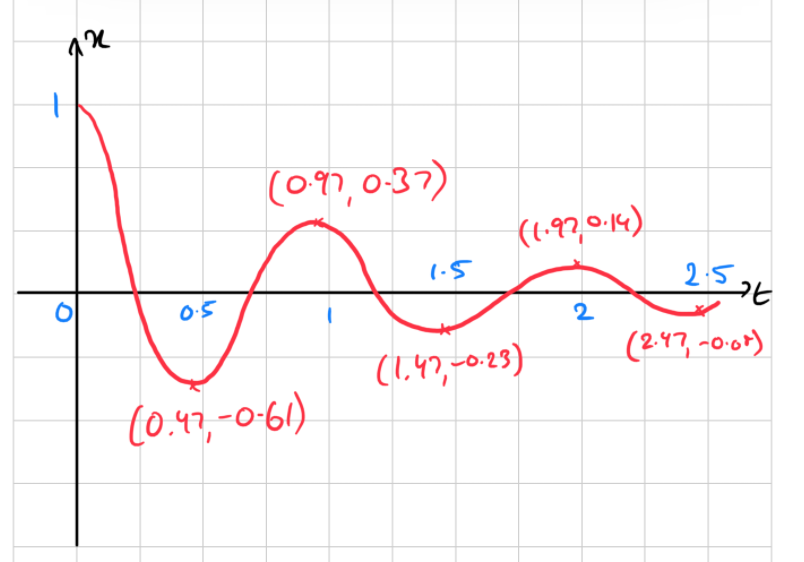
\includegraphics[width = 0.6\textwidth]{q1d.png}}
  \caption{Graph to show the solution of $x(t)$, when $a = -1$, $b = 2\pi$, $C=1$.}
\end{figure}
\subsection*{e}
Constants:
\begin{align}
  a &= - 1\\
  b &= 2\pi\\
  C &= 1
\end{align}
Derivatives:
\begin{align}
  x(t) &= Ce^{at}\cos{\left(bt\right)}\\
  x(0.5) &= -e^{0.5}\\
  x'(t) &= aC e^{at}\cos{\left(bt\right)} - bCe^{at}\sin{\left(bt\right)}\\
  x'(0.5) &= e^{-0.5}\\
  x''(t) &= a^2 C e^{at} \cos{\left(bt\right)} - abCe^{at}\sin{\left(bt\right)} - \left[ abCe^{at} + b^2 C e^{at}\cos{\left(bt\right)} \right]\\
  x''(0.5) &= -e^{0.5} + 4\pi^2e^{-0.5}
\end{align}
Final equation:
\begin{gather}
  x(t) \approx -e^{-0.5} + e^{-0.5}\left(t - 0.5\right) + \frac{-e^{-0.5}+ 4\pi^2e^{-0.5}}{2} \left(t-0.5\right)^2 + ...
\end{gather}
\begin{figure}[H]
  \centerline{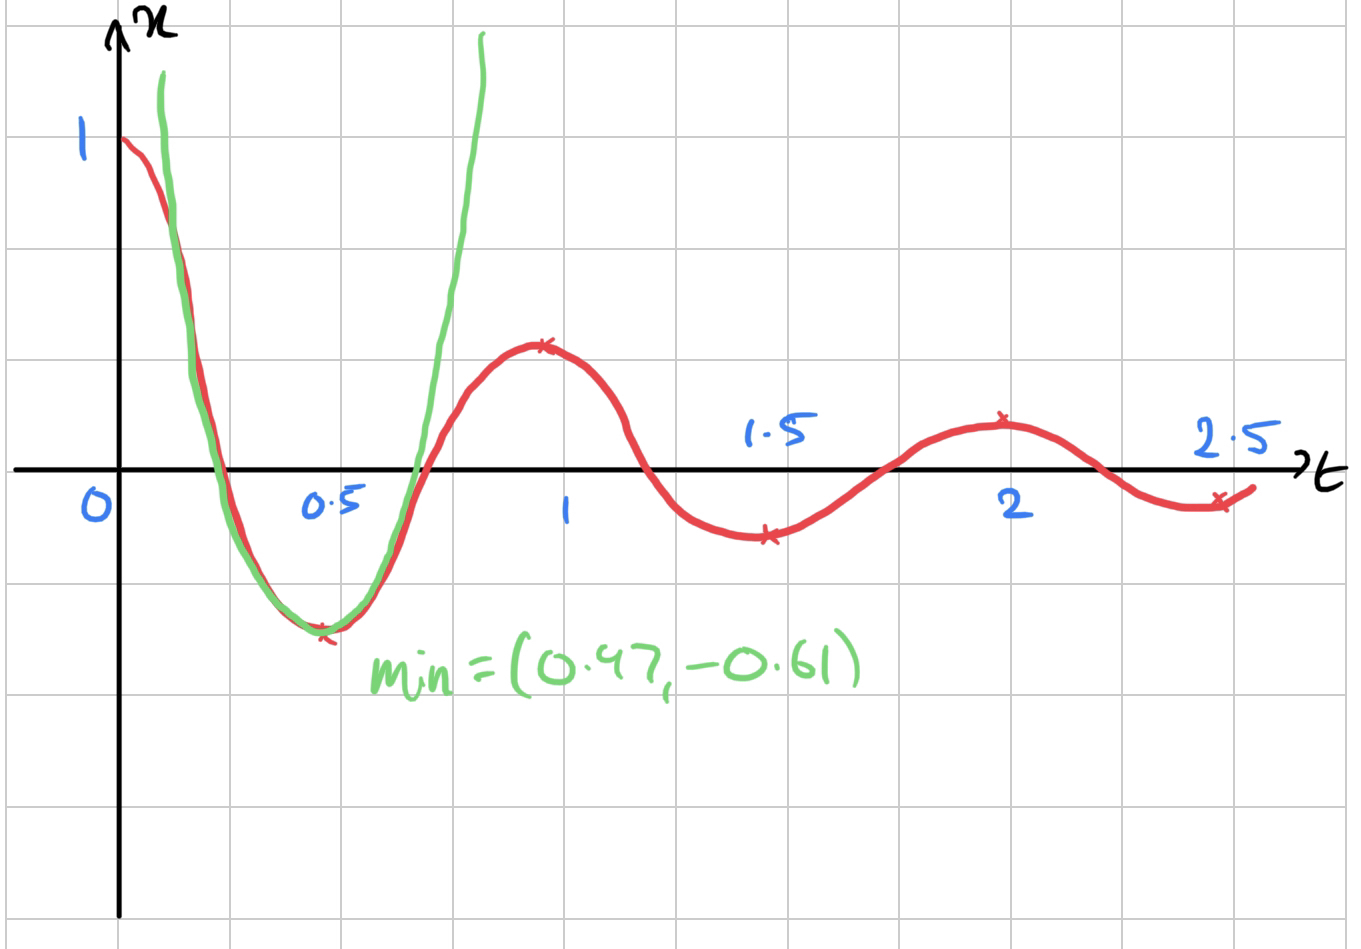
\includegraphics[width = 0.6\textwidth]{q1e.png}}
  \caption{Graph to show the solution of $x(t)$, when $a = -1$, $b = 2\pi$, $C=1$ (red), alongside Taylor series approximation (green).}
\end{figure}
\section{Question 2}
Boundary conditions:
Assuming a solution such that $u(x, y) = X(x)Y(y)$, $X(x) = X$ and $Y(y) = y$:
\begin{gather}
  Y \frac{d^2X}{dx^2} + X\frac{d^2 Y}{dy^2} = 0\\
  -\frac{1}{X}\frac{d^2X}{dx^2} = \frac{1}{Y}\frac{d^2 Y}{dy^2} = k
\end{gather}
\subsection*{For a positive constant}
Solving $X(x)$:
\begin{gather}
  \frac{1}{X}\frac{d^2X}{dx^2} = -k\\
  \frac{d^2X}{dx^2} + kX = 0\\
  m^2 + k = 0\\
  m = \pm i\sqrt{k}\\
  \textrm{Let } k = k_1^2\\
  X(x) = A\cos{\left(k_1 x\right)} + B\sin{\left(k_1 x\right)}\\
\end{gather}
Solving $Y(y)$:
\begin{gather}
  \frac{1}{Y}\frac{d^2 Y}{dy^2} = k\\
  \frac{d^2 Y}{dy^2} - kY = 0\\
  m^2 - k_1^2 = 0\\
  m = \pm \sqrt{k_1^2}\\
  Y(y) = C'e^{k_1 y} + D'e^{-k_1 y}\\
  Y(y) = C \cosh{\left(k_1 y\right)} + D \sinh{\left(k_1 y\right)}
\end{gather}
Hence for positive constant $k$:
\begin{gather}
  u_1(x,y) = \left[ A\cos{\left(k_1 x\right)} + B\sin{\left(k_1 x\right)} \right] \cdot \left[ C \cosh{\left(k_1 y\right)} + D \sinh{\left(k_1 y\right)} \right]
\end{gather}
\begin{table}[H]
  \begin{center}
  \begin{tabular}{|c|c|}
  \hline
  At $x = 0$ & $\frac{\partial u}{\partial x} = 0$\\
  \hline
  At $x = a$ & $\frac{\partial u}{\partial x} = 0$\\
  \hline
  At $x =0$ & $u = 0$\\
  \hline 
  At $y = b$ & $u = f(x)$\\
  \hline
  \end{tabular}
  \caption{Boundary conditions}
  \end{center}
\end{table}
Hence, for $y = 0$, $u = 0$ leading to $X(x) Y(y) = 0$. When $y = 0$, $\cosh{0} = 1$, $\sinh(0) = 0$, hence:
\begin{gather}
  u_1 (x, 0) = \left[ A\cos{\left(k_1 x\right)} + B\sin{\left(k_1 x\right)} \right] \cdot \left[ C \right] = 0
\end{gather}
We see here that $C$ must be 0. At $x = 0$, $\frac{du}{dx} = 0$:
\begin{gather}
  \left. \frac{du}{dx} \right|_{x = 0} = \left[ -Ak_1 \sin{\left(k_1 x\right)} + B k_1 \cos{\left(k_1 x\right)} \right] \cdot \left[ D \sinh{k_1 y} \right] = 0\\
  -Ak_1 \sin{\left(k_1 x\right)} = 0\\
  \cos{\left(k_1 x\right)} = 0
\end{gather}
We see here that $B$ must be 0. At $x = a$, $\frac{du}{dx} = 0$:
\begin{gather}
  \left. \frac{du}{dx} \right|_{x = a} = \left[ -Ak_1 \sin{\left(k_1 x\right)} \right] \cdot \left[ D \sinh{k_1 y} \right] = 0
\end{gather}
If $A$ or $D = 0$, we get a trivial solution. Hence:
\begin{gather}
  \sin{\left(k_1 a\right)} = 0
\end{gather}
Hence:
\begin{gather}
  u_1(x,y) = \left[ A\cos{\left(k_1 x \right)}\right]\cdot \left[ D\sinh{k_1 y} \right]
\end{gather}
\end{document}